\documentclass[11pt,a4paper]{article}
\usepackage[T1]{fontenc}
\usepackage{lmodern}
\usepackage[margin=2.5cm]{geometry}
\usepackage{amsmath,amssymb}
\usepackage{graphicx}
\usepackage{booktabs}
\usepackage{array}
\usepackage[font=small,labelfont=bf]{caption}
\usepackage{xcolor}
\usepackage[colorlinks=true,linkcolor=blue!50!black,citecolor=blue!50!black,urlcolor=blue!50!black]{hyperref}

\graphicspath{{figs/}}
\newcommand{\tm}[1]{\texttt{\detokenize{#1}}}   % a machine string
\newcommand{\BB}[1]{BB(#1)}
\sloppy

\title{Growth laws of small Turing machines\\[2pt]
\large What fitted formulas reveal about busy beaver machines}
\author{An exploratory study with \texttt{basin}}
\date{23--25 November 2026}

\begin{document}
\maketitle

\begin{abstract}
We simulated small Turing machines from a blank tape, recorded how far the head has
spread (the \emph{span}) over time, and asked the symbolic-regression tool \texttt{basin} for
a formula $\mathrm{span}(t)$. The machines studied are all non-halting 3-state machines, uniform
samples of 20,000 non-halting 4- and 5-state machines, the 608 \BB{6} holdouts, the named \BB{6}
cryptids, Skelet's 43 \BB{5} machines and \BB{5} halters. The results, in the order the report
develops them:
(1)~The fitted laws fall into a few sharp growth classes (linear, bounded, $\sqrt t$, $\log t$,
and a rare $t^{1/3}$) in nearly the same shares for 3, 4 and 5 states.
(2)~The fitted constants are exact numbers that identify each machine's mechanism: rational speeds
that obey a parity rule, rational $c^2$ for bouncers, and counters in exact algebraic bases,
including 15,054 \BB{5} records that count in base $\varphi$.
(3)~Reading counters' values off the tape shows 67 distinct \BB{5} behaviours counting in the
rational base $3/2$, which refutes the hypothesis that small machines count only in Pisot bases.
(4)~How roughly \texttt{basin} fits a machine separates hard machines from easy ones, but not
halting from non-halting machines.
(5)~The \BB{5} champion's fitted constant $1.920$ follows from its Collatz-like rule, and all of
its roughness is a wobble that repeats on a log scale of time.
(6)~Such a wobble marks machines whose macro steps \emph{multiply} their size. Its period, or the
span ratio between its teeth, measures the multiplier: Antihydra's $3/2$ was predicted from its
rule and then measured, and the cryptids give $3/2$, $4/3$ and $8/3$, confirmed on their tapes.
Unlike a bouncer's, the wobble does not fade as the machine grows. Of all 2.77 million
$\sqrt t$-like \BB{5} records, 34,956 (1.26\%) share this scale invariance, a label that does not
change between $2^{24}$ and $2^{26}$ steps.
(7)~Reading the macro rule off the tape splits these machines in two: exponential counters with
an integer multiplier and one exact formula (for example $n \to 2n+6$), and Collatz-like machines
with a fractional multiplier and an exact formula for each residue of $n$. \BB{5} contains at least
2,196 distinct Collatz-like behaviours, with multipliers $3/2$, $4/3$, $5/2$, $5/4$, $5/3$, $7/4$ and
$8/3$: the champion's multiplier and every cryptid multiplier except $9/8$. The three views agree: the
six roughest of 638 census $\sqrt t$ machines are exactly the six scale-invariant ones, four
doublers and two Collatz-like.
\end{abstract}

\paragraph{Status.} Exploratory, not pre-registered. The classification rules
(Section~\ref{sec:pipeline}) were fixed while looking at partial results. The census numbers
(Sections~\ref{sec:classes}, \ref{sec:constants} and~\ref{sec:bb6}) are recomputed from the committed
files by \texttt{busy\_beaver/analyze.py}. The later analyses are reproduced by the scripts in
\texttt{busy\_beaver/pisot/} (base $3/2$), \texttt{wobble/} (log-periodic wobble), \texttt{collatz/}
(cryptid rules, scale invariance, rules read from the tape) and \texttt{screen/} (the \BB{5}
screen); see Section~\ref{sec:repro}. The \BB{5} screen in Section~\ref{sec:screen} covers all 2.77 million
$\sqrt t$-like records; its rule test (Section~\ref{sec:fullrules}) reads every behaviour except the
two largest groups. A fitted
law describes a machine on the window it was fitted on and says nothing about what happens later:
the \BB{5} champion fits $1.92\sqrt t$ cleanly and halts at step 47,176,870.

\tableofcontents

%=================================================================================================
\section{Background}

A Turing machine here has $n$ states, two symbols and one tape, and starts in state A on a blank
(all-zero) tape. A machine is written as a string of $n$ blocks, one per state, each holding
two transitions (for read symbols 0 and 1) of the form \emph{write, move, next state}; for
example \tm{1RB1LC} means ``on 0 write 1, move right, go to B; on 1 write 1, move left, go to C''.
A transition \tm{---} (or a target outside the states) halts. The busy beaver value $S(n)$ is
the largest number of steps taken by a halting $n$-state machine; $S(5) = 47{,}176{,}870$ was
proved by the bbchallenge collaboration in 2024, and \BB{6} remains open, with 608 holdout
machines (up to equivalence) whose behaviour is undecided as of October 2026.

The bbchallenge \emph{zoology} names the common non-halting behaviours. A \emph{cycler} repeats a
configuration exactly; its span is bounded. A \emph{translated cycler} repeats a pattern that
shifts along the tape, so its span grows linearly. A \emph{bouncer} sweeps back and forth over a
region that grows by a fixed amount per sweep, so its span grows like $\sqrt t$. A \emph{counter}
implements an odometer on the tape, so its span grows like $\log t$. \emph{Cryptids} are machines
whose halting is equivalent to an open Collatz-like problem. \emph{Skelet's 43 machines} are the
\BB{5} machines that Skelet's search program could not decide; all were later proven non-halting,
several with individual proofs, and they serve here as hard controls.

\texttt{basin} is a symbolic-regression library (this repository, PyPI \texttt{basin-sr}). Given
data $(x, y)$ it searches small formulas (sums, powers with denominators 1, 2, 3, and rational
functions with up to five free coefficients) and returns the law with the best cross-validated
error, together with that error.

%=================================================================================================
\section{Data}

\begin{table}[h]
\centering\small
\begin{tabular}{@{}p{3.0cm}p{6.2cm}p{4.9cm}@{}}
\toprule
set & source & used \\
\midrule
\BB{5} & bbchallenge seed database (88,664,064 records: 14,322,029 time-limit, then 74,342,035
space-limit; all proven non-halting) & uniform sample of 20,000 (seed 0); all 14,322,029
time-limit records for the counter census and the screen of Section~\ref{sec:screen} \\
\BB{4} & own tree enumeration, \texttt{small/enum.c}: 436,278 non-halting machines & uniform sample of 20,000 (seed 0)\\
\BB{3} & own tree enumeration: 2,678 non-halting machines & all \\
\BB{6} holdouts & bbchallenge wiki, \texttt{BB6\_holdouts\_608.txt} (30 Oct 2026) & all 608\\
\BB{6} cryptids & bbchallenge wiki (read 23 Nov 2026) & 20 cryptids, 6 potential cryptids \\
\BB{6} champion & bbchallenge wiki & 1 machine ($\approx 10\uparrow\uparrow10\uparrow\uparrow10\uparrow\uparrow8$ steps)\\
\BB{5} top halters & bbchallenge wiki, Top Halters table & 20 machines, 2.36M--47.2M steps\\
Skelet's machines & bbchallenge wiki, Skelet's 43 holdouts & all 43, as controls\\
random 6-state & \texttt{bb6/rand6.c}: one halting slot, other transitions uniform; machines that visit all 6 states and survive $2^{16}$ steps & 5,000 fitted \\
\BB{5} halters & \texttt{halt/enum\_halt.c}: tree leaves halting between $2^{12}$ and $2^{16}$ steps & all 118 \\
\bottomrule
\end{tabular}
\caption{Machine sets. The tree enumeration uses bbchallenge's normal form (first transition
\tm{1RB}, states introduced in order) and was checked against the known $S(2)$, $S(3)$, $S(4)$.
Counts are per record: records that differ only in transitions a machine never uses are counted
separately, as in the bbchallenge database.}
\label{tab:data}
\end{table}

Table~\ref{tab:data} lists the machine sets.

\paragraph{Measurement.} The dependent variable is the span: the number of cells from the leftmost
to the rightmost cell visited so far, inclusive. It is recorded at 49 checkpoints
$t_k = \mathrm{round}(2^{10 + k/4})$, $k = 0,\dots,48$, from $2^{10}$ to $2^{22} = 4{,}194{,}304$
steps. The fits use $k = 8,\dots,48$ (41 points, $2^{12}$ to $2^{22}$). Two C simulators were
used (one reads database records, one reads machine strings); both reproduce the \BB{5}
champion's 47,176,870 steps exactly, and every top halter halts at exactly its published step.

%=================================================================================================
\section{Method}
\label{sec:pipeline}

\subsection{Fitting and classification}
\begin{enumerate}
\item \textbf{Simulate} each machine for $2^{22}$ steps and record the span at the 49 checkpoints.
\item \textbf{Bounded:} if the span is the same at all 41 fit checkpoints, the class is
\emph{bounded} and \texttt{basin} is not called.
\item \textbf{Fit twice} with \texttt{basin.discover} at default settings (\texttt{MAX\_FREE}=5,
\texttt{EXHAUSTIVE\_TERMS}=4, $5{\times}5$ cross-validation): span against $t$, and span against
$u = \log_2 t$ (\texttt{basin} has no logarithm, so $a\log t + b$ appears as $au+b$).
\item \textbf{Roughness} is \texttt{basin}'s cross-validated relative mean squared error of the
chosen law.
\item \textbf{Choose a law} (rules fixed during the study):
a $u$-law is allowed only if the span grew slower than $t^{0.4}$ between $2^{20}$ and $2^{22}$;
if the two errors are within a factor 2, the law with fewer coefficients wins; otherwise the
lower error wins. Without the first rule 3 clean $\sqrt t$ machines were labelled $\log$; without
the second, 116.
\item \textbf{Class:} a $u$-law gives $\log$. Otherwise the local exponent
$d\ln \mathrm{span}/d\ln t$ of the law at $t = 2^{22}$ is rounded to $0, \tfrac13, \tfrac12,
\tfrac23$ or $1$ if within $0.04$, and labelled \emph{other} if not.
\item \textbf{Rate:} $f(t)/t$ for linear laws, $f(t)/t^p$ for $t^p$ laws, $f(22.5)-f(21.5)$ (cells
per doubling of $t$) for $\log$ laws, and the span itself for bounded machines.
\end{enumerate}

\subsection{Counter census}
\label{sec:countermethod}
The base of a counter is measured from timing, not from the fit:
\begin{enumerate}
\item Scan all 14,322,029 time-limit \BB{5} records for $2^{16}$ steps. Records whose span slope
between $2^{14}$ and $2^{16}$ lies in $(0, 0.25]$ are counter candidates: 297,225 records.
\item Run each candidate to $2^{24}$ steps and record every step at which the span grows.
\item The \emph{time factor per new cell} is $(t_b/t_a)^{1/q}$ over the last $q$ increments after
$2^{14}$ steps, with $q$ a multiple of 6 (this cancels repeating patterns of length 1, 2 and 3).
\end{enumerate}
A counter in base $\beta$ that uses $k$ cells per digit gains a cell each time $t$ grows by
$\beta^{1/k}$, so the factor identifies $\beta^{1/k}$; the values were matched against a list of
candidate constants with tolerance $10^{-3}$.

\subsection{Reading the base off the tape}
\label{sec:weightmethod}
Timing identifies only $\beta^{1/k}$, and only among constants that were put on the candidate
list. A direct test reads the counter's value from the tape:
\begin{enumerate}
\item Run the machine and take a snapshot of the tape each time the head arrives at a fixed
cell $k$ (searched over $k = 0,\dots,7$) counted from one end of the visited region. Number the
snapshots $n = 0, 1, 2, \dots$; for a counter each snapshot is one increment.
\item Index the cells $x_0, x_1, \dots$ from that end and fit, by least squares over the last
75\% of the snapshots,
\[ n \;=\; c + \sum_i w_i\, x_i . \]
\item A counter in a positional system with a fixed digit encoding fits \emph{exactly}
(residual at rounding level), and the weights $w_i$ are the place values. Their ratio gives
the base with no candidate list.
\end{enumerate}
The method was validated on known counters (Figure~\ref{fig:weights}): a binary machine gives
weights $1, 2, 4, 8, \dots$ exactly, and a base-$\varphi$ machine gives
$1.5, 2.5, 4, 7, 11, 18, 29, 47, \dots$ (Lucas numbers, ratio $\to\varphi$), the binary fit with residual
below $10^{-8}$ and the $\varphi$ fit exact to within half an increment.

%=================================================================================================
\section{Growth classes}
\label{sec:classes}

\begin{figure}[t]
\centering
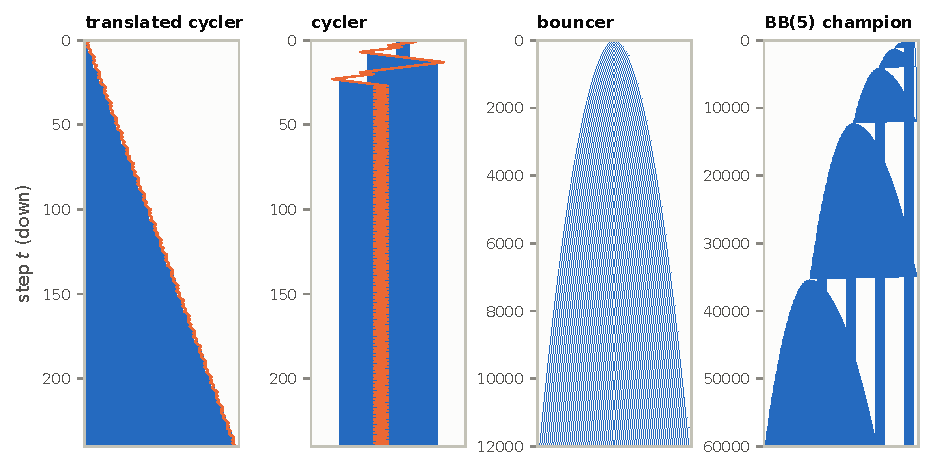
\includegraphics[width=\textwidth]{spacetime}
\caption{Space-time diagrams (time runs down, cells with a 1 in blue, head in orange where every
step is drawn). From left: a translated cycler (240 steps), a cycler (240 steps), a bouncer
(12,000 steps, every 12th row), and the \BB{5} champion (60,000 steps, every 40th row), whose
sweeps start over at a larger size after each macro step of its Collatz-like rule.}
\label{fig:spacetime}
\end{figure}

\begin{figure}[t]
\centering
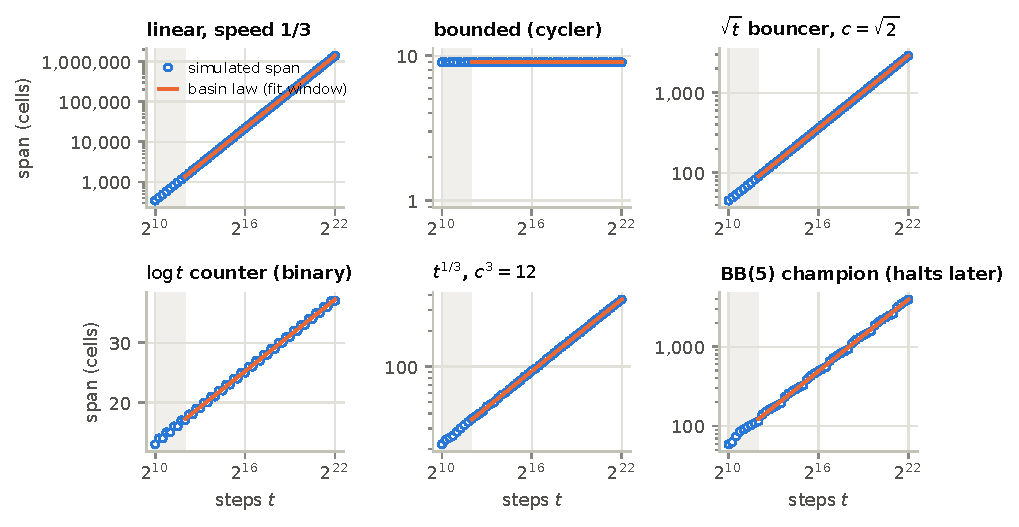
\includegraphics[width=\textwidth]{span_examples}
\caption{Span against steps for one machine per class, with \texttt{basin}'s law over the fit
window $2^{12}$--$2^{22}$ (unshaded). The counter panel has a linear vertical axis, so its
$\log t$ law is a straight line. The champion's steps are the macro steps of its rule; it halts
at 47,176,870, after this window.}
\label{fig:spanex}
\end{figure}

\begin{figure}[t]
\centering
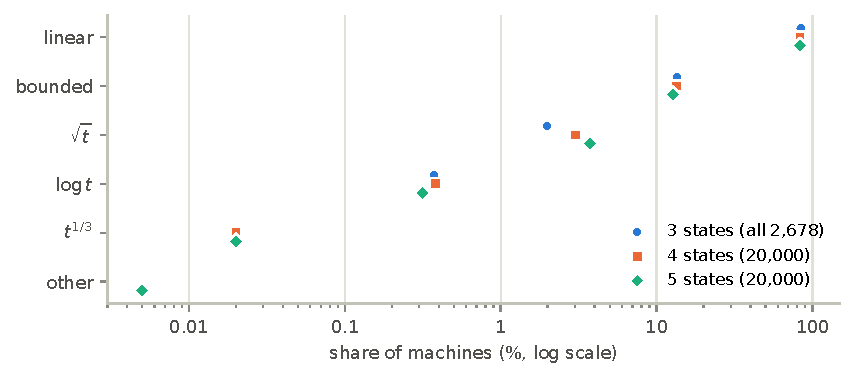
\includegraphics[width=\textwidth]{classes}
\caption{Share of machines in each growth class, window $2^{12}$--$2^{22}$. The shares are
nearly the same for 3, 4 and 5 states.}
\label{fig:classes}
\end{figure}

\begin{table}[h]
\centering\small
\begin{tabular}{@{}lrrrrr@{}}
\toprule
growth class & 3 states & 4 states & 5 states & 5 states, & 5 states, \\
 & (2,678) & (20,000) & (20,000) & time limit (3,259) & space limit (16,741)\\
\midrule
linear (translated cyclers) & 84.2\% & 83.2\% & 83.1\% & -- & 99.3\% \\
bounded (cyclers) & 13.5\% & 13.4\% & 12.8\% & 78.4\% & -- \\
$\sqrt t$ (bouncers) & 2.0\% & 3.0\% & 3.7\% & 19.6\% & 0.7\% \\
$\log t$ (counters) & 0.4\% & 0.4\% & 0.3\% & 1.9\% & -- \\
$t^{1/3}$ & -- & 0.02\% (4) & 0.02\% (4) & 0.1\% & -- \\
other & -- & -- & 1 machine & -- & 1 machine \\
\bottomrule
\end{tabular}
\caption{Growth classes. 95\% margins with 20,000 machines are about $\pm0.5$ points on linear
and bounded, $\pm0.26$ on $\sqrt t$ and $\pm0.08$ on $\log t$. The time-limit/space-limit split
in the database is a split by class, as expected from how the database was built.}
\label{tab:classes}
\end{table}

The machines fall into a handful of sharp classes (Table~\ref{tab:classes},
Figures~\ref{fig:spacetime}--\ref{fig:classes}), and the shares hardly change from 3 to 5 states.
No sampled \BB{5} machine has a raw slope between $0.15$ and $0.25$ or between $0.55$ and $0.95$.
With 20,000 machines this only bounds those gaps below about $0.015\%$ of the database, and the
rare $t^{1/3}$ class shows that intermediate exponents do exist.

The single \emph{other} machine, \tm{1RB---_1LC1RA_0RB0RD_1RC1LE_0LD1RC}, multiplies its span by a
repeating cycle of factors ($\times1.97, 1.46, 1.42, 1.42$) every $32\times$ in time, which
averages $t^{0.51}$: it is $\sqrt t$ with a wobble that repeats on a log scale, for which
\texttt{basin} has no term.

%=================================================================================================
\section{The constants are exact}
\label{sec:constants}

\subsection{Linear speeds and a parity rule}
A translated cycler repeats a $p$-step pattern that shifts by $d$ cells, so its speed is $d/p$.
The head moves one cell every step, so \textbf{$p \equiv d \pmod 2$}. A speed $a/b$ in lowest
terms with $a+b$ even can have period $b$; with $a+b$ odd the period must be at least $2b$,
a longer and rarer pattern. In the \BB{5} sample, 11,465 linear machines have $a+b$ even and
3,362 have $a+b$ odd. The commonest speeds are $1/3$ (2,758), $1$ (2,665), $1/5$ (2,064) and
$1/7$ (1,266) (Figure~\ref{fig:speeds}).

\begin{figure}[t]
\centering
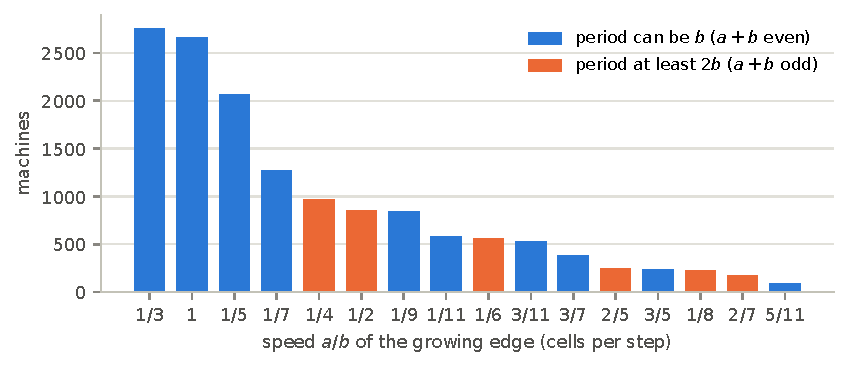
\includegraphics[width=\textwidth]{speeds}
\caption{The 16 commonest speeds among linear \BB{5} machines, coloured by whether the speed's
shortest possible period is $b$ or $2b$.}
\label{fig:speeds}
\end{figure}

\subsection{Bouncers: rational $c^2$}
If a bouncer's region grows by $a$ cells per round trip and the head sweeps at $h$ cells per step,
then after $n$ round trips $t \approx a n^2/h$ and $\mathrm{span} \approx a n$, so
$\mathrm{span}\approx c\sqrt t$ with
\[ c^2 = a\,h . \]
Both factors are simple rationals, so $c^2$ should be one too. Of the 749 $\sqrt t$ machines in
the \BB{5} sample, 60.5\% have $c^2$ within 0.2\% of a fraction with denominator at most 6,
against 11.5\% for random values spread over the same range; at denominator $\le4$ and
0.1\% tolerance the figures are 28.3\% against 2.9\%. The commonest value is $c^2 = 2$ (one new
cell at each end per round trip, at full speed), followed by $1, 4/3, 4, 3/2, 8/3, 2/3, 3$
(Figure~\ref{fig:bouncers}).

\begin{figure}[t]
\centering
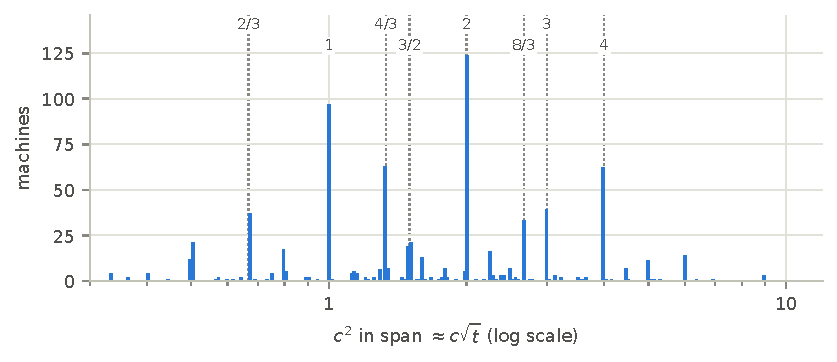
\includegraphics[width=\textwidth]{bouncers}
\caption{Distribution of $c^2$ for the 749 $\sqrt t$ machines in the \BB{5} sample. The mass sits
on simple fractions (dashed).}
\label{fig:bouncers}
\end{figure}

\subsection{The $t^{1/3}$ class}
Three 4-state machines have $c \approx 1.4424 \approx 3^{1/3}$ (fitted $c^3 = 3.02$--$3.06$). Two
5-state machines share the law $2.2895\,t^{1/3} - 0.979$, and $2.2895^3 = 12.00$. A third 5-state
machine has $c^3 = 23.8$, close to 24. A plausible mechanism is a round of growth that costs time
proportional to the span squared, which gives $c^3 = 3\times$(a simple ratio); this has not been
derived for any machine.

\subsection{Counters count in exact algebraic bases}
Table~\ref{tab:bases} and Figure~\ref{fig:bases} give the time factor per new cell for all
297,225 \BB{5} counter candidates. Most are binary or ternary with 1 to 6 cells per digit. A
sizeable minority count in irrational bases: \textbf{15,054 records count in base $\varphi$}
(Fibonacci/Zeckendorf numeration, where place values are Fibonacci numbers and no two adjacent
digits are 1), and others count in the plastic number, its square, the tribonacci constant,
Narayana's cows constant, and $1+\sqrt2$ (Pell). The matches are tight: median relative error
$7\times10^{-5}$ for $\varphi$, $1.9\times10^{-5}$ for tribonacci, $1.2\times10^{-5}$ for the
plastic number squared. The four $\varphi$ machines in the 20,000 sample, run to $2^{32}$ steps,
match to $10^{-6}$.

Revisiting the unidentified values gave three more identifications:
\begin{itemize}
\item The cluster at $1.84778$ (189 records) is $\sqrt{2+\sqrt2} = 2\cos(\pi/8) = 1.847759$
(median relative error $1.1\times10^{-5}$): base $2+\sqrt2$ with 2 cells per digit.
\item The large cluster at $1.36083$ (4,718 records, 10--90\% range $1.36072$--$1.36094$) matches
$2^{4/9} = 1.360790$ (relative error $2.6\times10^{-5}$), perhaps base 16 with 9 cells per digit.
About 2,000 candidates were tried, so this could be a chance match; it has not been checked on
the tape.
\item 97 records at $\sqrt{3/2}$: \textbf{rational base $3/2$}, confirmed on the tape in
Section~\ref{sec:base32}. Eight more records sat at $3/2$ per cell at $2^{24}$ steps, but longer
runs show they have no fixed base (Section~\ref{sec:long}).
\end{itemize}

\begin{table}[t]
\centering\small
\begin{tabular}{@{}llrr@{}}
\toprule
time factor per new cell & meaning & records & distinct growth sequences \\
\midrule
$\sqrt2$ & binary, 2 cells per digit & 140,307 & 31,636\\
$2$ & binary, 1 cell per digit & 81,492 & 11,011\\
$2^{1/3}$ & binary, 3 cells per digit & 31,439 & 12,770\\
$\varphi = 1.618034$ & Fibonacci, $x^2=x+1$ & 15,054 & 4,235\\
$2^{1/4}$ & binary, 4 cells per digit & 6,880 & 3,883\\
$\sqrt3$ & ternary, 2 cells per digit & 5,631 & 2,024\\
$2^{4/9} = 1.360790$ & candidate, unchecked & 4,718 & 2,927\\
$2^{2/3}$ & binary, 3 cells per 2 digits & 3,102 & 1,332\\
$3^{1/3}$ & ternary, 3 cells per digit & 1,623 & 851\\
$\sqrt\varphi$ & Fibonacci, 2 cells per digit & 614 & 388\\
$1.465571$ & Narayana, $x^3 = x^2+1$ & 476 & 309\\
$1.324718$ & plastic, $x^3 = x+1$ & 338 & 209\\
$\sqrt{1+\sqrt2}$ & Pell, 2 cells per digit & 302 & 192\\
$\sqrt{2+\sqrt2} = 1.847759$ & $x^2 = 4x - 2$, 2 cells per digit & 189 & 148\\
$1.754878$ & plastic squared & 184 & 134\\
$2^{1/6}, 3^{1/4}, 2^{1/5}$ & more cells per digit & 138, 124, 12 & \\
$1.839287$ & tribonacci, $x^3=x^2+x+1$ & 101 & 53\\
$\sqrt{3/2}$ & \textbf{rational base 3/2}, 2 cells per digit & 97 & 67\\
$\varphi^{1/3}$ & Fibonacci, 3 cells per digit & 27 & 23\\
$\approx1.5$ & irregular, no fixed base (Sec.~\ref{sec:long}) & 8 & 1 behaviour\\
unidentified & & 4,369 & \\
\bottomrule
\end{tabular}
\caption{Time factor per new cell for the 297,225 \BB{5} counter candidates, with the three new
identifications. ``Distinct growth sequences'' counts distinct exact lists of increment times, a
ceiling on the number of distinct behaviours. Some of the remaining unidentified values sit just
off $\sqrt2$ and look like binary counters that have not settled by $2^{24}$ steps.}
\label{tab:bases}
\end{table}

\begin{figure}[t]
\centering
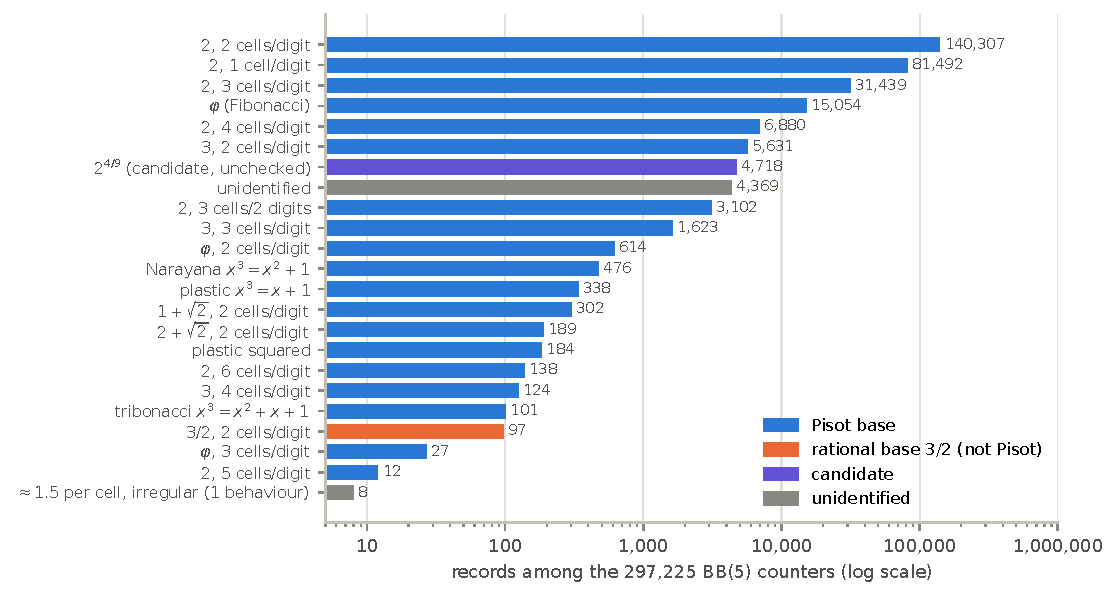
\includegraphics[width=\textwidth]{bases}
\caption{Records per counting base among the 297,225 \BB{5} counters (log scale). Every
identified irrational base is a Pisot number; the rational base $3/2$ (orange) is not. The
8 records near $1.5$ per cell (grey) have no fixed base.}
\label{fig:bases}
\end{figure}

%=================================================================================================
\section{Rational base 3/2 and the Pisot hypothesis}
\label{sec:base32}

\subsection{The hypothesis}
Every irrational base found by the first census is a \emph{Pisot number}: an algebraic integer
greater than 1 whose other conjugates all lie strictly inside the unit circle. Frougny showed
that normalisation in base $\beta$ can be done by a finite automaton when $\beta$ is a Pisot
number, and a small Turing machine is a finite automaton sweeping a tape. This suggested that
small machines might only be able to count in Pisot bases, and a counter in a non-Pisot base
would refute it. The base $3/2$ is not an algebraic integer, so it is not Pisot.

\subsection{Reading the base-3/2 machines}
\begin{figure}[t]
\centering
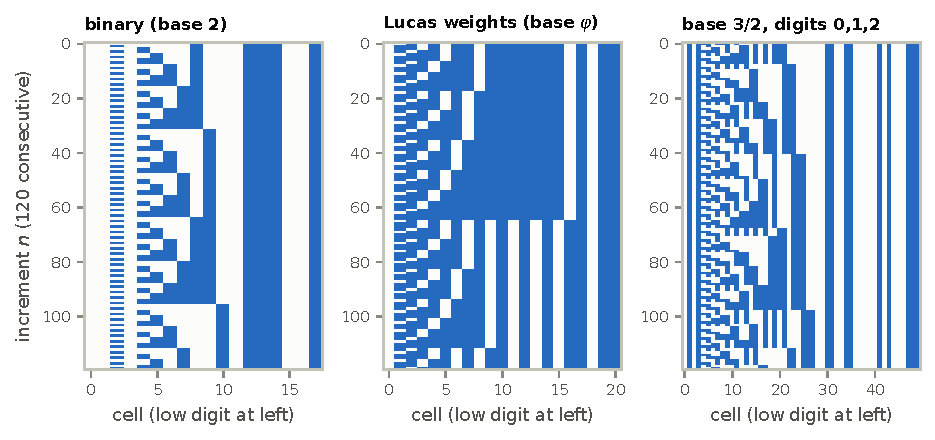
\includegraphics[width=\textwidth]{counters_tape}
\caption[Counter tapes at consecutive increments]{The counter's tape at 120 consecutive increments, low digit at the left, for a binary
machine, a base-$\varphi$ machine and a base-$3/2$ machine
(\tm{1RB1RA_1LC0RD_---1LD_0LE1LE_0RA0LD}). Binary shows the familiar ruler pattern; base $3/2$
shows carries of irregular length.}
\label{fig:countertape}
\end{figure}

\begin{figure}[t]
\centering
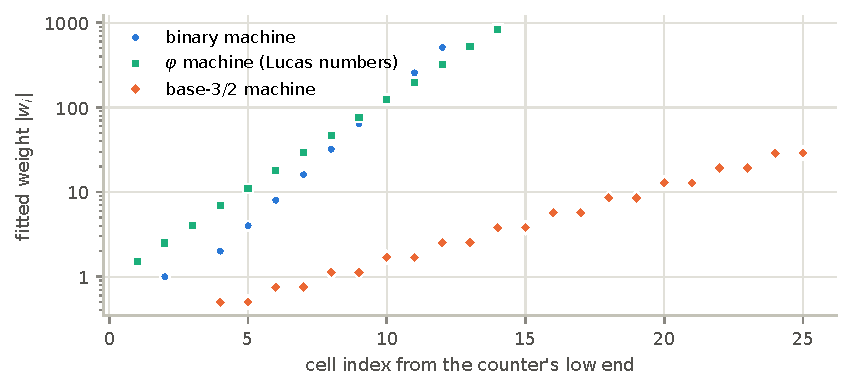
\includegraphics[width=\textwidth]{weights}
\caption{Place values read off the tape by the regression of Section~\ref{sec:weightmethod}.
Binary: $1, 2, 4, \dots$. Base $\varphi$: Lucas numbers $4, 7, 11, 18, \dots$. Base $3/2$: equal
weights in pairs, $\tfrac12(\tfrac32)^j$, each pair exactly $3/2$ times the one before. All
three fits are exact.}
\label{fig:weights}
\end{figure}

Figure~\ref{fig:countertape} shows what such a counter looks like on the tape. The weight
regression was run on one representative of each of the 67 distinct growth sequences
at $\sqrt{3/2}$:
\begin{itemize}
\item \textbf{All 67 fit exactly.} The maximum residual is below $10^{-8}$ over $2\times10^4$ to
$8\times10^4$ increments (64 with the trigger at the end cell, 3 with the trigger 3, 4 or 7 cells
in from the end).
\item \textbf{In all 67, place values grow by exactly $3/2$ per two cells} (median ratio
$1.50000$ over the middle cells).
\item At least two digit encodings occur. In
\tm{1RB1RA_1LC0RD_---1LD_0LE1LE_0RA0LD} each pair of cells is a digit $d_j\in\{0,1,2\}$ (its
number of 1s) and
\[ n = c + \sum_j \tfrac{d_j}{2}\left(\tfrac32\right)^j , \]
which is exactly the rational base numeration system of Akiyama, Frougny and Sakarovitch.
In \tm{1RB---_0RC0LB_1LD0RE_1LB1RE_1LC1RD} a pair of cells has weights
$(-\tfrac12, \tfrac32)\cdot(\tfrac32)^j$: the cell pairs 00, 10, 11, 01 are the digits
$0, -1, 2, 3$ in units of $\tfrac12(\tfrac32)^j$, a redundant signed-digit version of the same base.
\end{itemize}

Adding 1 in base $3/2$ needs only a bounded carry: add 2 to the lowest digit; while a digit
reaches 3 or more, subtract 3 from it and add 2 to the next. A finite-state machine sweeping the
digits once can do this, so base $3/2$ is as easy for a small machine as binary.
Frougny's theorem concerns base-$\beta$ numeration with integer digits and does not cover
rational bases, so it was never evidence against them.

\paragraph{The 8 records at $3/2$ per cell} are a different mechanism. Each repeatedly counts up
inside a fixed region, overflows, zeroes the region, and starts again in a region one cell longer.
The weight regression fails for them (residual in the thousands), even within a single counting
phase and with products of neighbouring cells added as features, so the count is not stored in a
fixed linear code. All eight share one behaviour after the first few increments. The long runs in
Section~\ref{sec:long} show that their growth factor is not constant, so the match to $3/2$ at
$2^{24}$ steps was a coincidence of that window. Their mechanism is unresolved.

\subsection{Long runs}
\label{sec:long}
To check that the timing values are converging and not drifting, the 67 distinct $\sqrt{3/2}$
behaviours, the 8 records at $3/2$, and 5 control machines each from base 2, $\sqrt2$, $\varphi$,
plastic and Narayana were run to $2^{36} \approx 6.9\times10^{10}$ steps, recording every span
increment. Figure~\ref{fig:convergence} shows the median relative error of the time factor per
cell against the expected base, as a function of run length.

\IfFileExists{figs/convergence.pdf}{%
\begin{figure}[t]
\centering
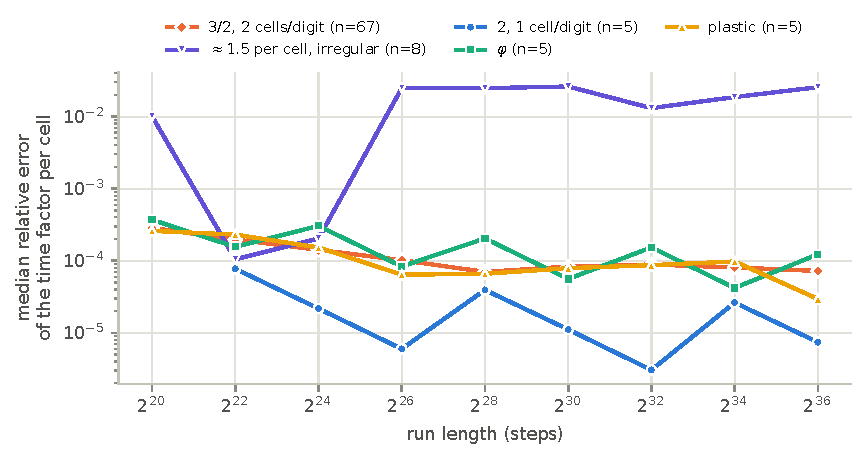
\includegraphics[width=\textwidth]{convergence}
\caption{Convergence of the time factor per new cell with run length (median over machines).}
\label{fig:convergence}
\end{figure}}{}

\begin{itemize}
\item \textbf{The 67 base-$3/2$ behaviours hold.} Median relative error against $\sqrt{3/2}$ is
$1.4\times10^{-4}$ at $2^{24}$ steps and $7\times10^{-5}$ at $2^{36}$, worst $2.1\times10^{-4}$;
this is the same level as the Pisot controls ($\varphi$: $1.2\times10^{-4}$; plastic:
$3\times10^{-5}$; base 2: $7\times10^{-6}$ at $2^{36}$).
\item The error falls slowly for every group, controls included, because the estimate uses the
last $q$ increments and $q$ grows only linearly in $\log t$; what remains is the counter's own
within-cycle unevenness, not drift.
\item \textbf{The eight records at $3/2$ per cell do not converge.} Their factor per cell is
$1.4998$ at $2^{24}$ but $1.537$, $1.520$ and $1.538$ at $2^{28}$, $2^{32}$ and $2^{36}$. The
ratios between successive increments are irregular (for example $1.345, 1.744, 1.857, 3.093$)
apart from a repeating $1, 1, 2$ motif, and the time between repeats of the motif grows by
$\times10.7, 17.8, 13.6, 10.7$. This looks like a Collatz-like process with average growth near
$1.5$ per cell, not a counter in a fixed base.
\end{itemize}

\subsection{What survives}
The hypothesis ``small machines count only in Pisot bases'' is \textbf{refuted}. A version
consistent with everything seen so far is: \emph{every base is either a Pisot number or a
rational number.} Rational bases other than $3/2$ were looked for and not found: no records lie
within $10^{-3}$ of $4/3$, $5/3$, $5/2$ or $\sqrt{4/3}$; 7 lie near $\sqrt{5/2}$ and have not been
checked. A cleaner test of the refined statement would apply the weight regression to every
counter, not only to those flagged by timing.

%=================================================================================================
\section{Roughness: hard machines, BB(6) and halting}
\label{sec:bb6}

The sections so far used the laws \texttt{basin} found. This one uses how well it found them: the
roughness of Section~\ref{sec:pipeline}, compared within each growth class.

\paragraph{The holdouts are a different population.} Random 6-state machines are 86.9\% linear and
11.9\% bounded, like \BB{3}--\BB{5}. The 608 holdouts are 37.2\% no simple law, 32.4\% $\sqrt t$,
16.9\% $\log t$, 8.6\% $t^{1/3}$, 3.1\% nearly flat, 1.5\% $t^{2/3}$ and 0.3\% linear. Their class
labels are less reliable: the share with a clean law is 75\% in the $\sqrt t$ class, 44\% in
$t^{1/3}$ and 16\% in $\log t$, and the 9 apparent $t^{2/3}$ machines are curving rational
functions, not clean powers. The $t^{1/3}$ class, 0.02\% of \BB{4} and \BB{5}, is 8.6\% of the
holdouts.

\paragraph{Roughness detects hard machines.} Every holdout is rougher than the 99th percentile of
the random 6-state machines (AUC 1.000) and of the \BB{5} census (AUC 0.999); within the $\sqrt t$
class the separation is clean (Figure~\ref{fig:roughness}). This is partly by construction: the
holdouts are what remains after bbchallenge's deciders removed cyclers, translated cyclers,
bouncers and counters, which are exactly the machines \texttt{basin} fits smoothly.

\paragraph{Roughness does not detect halting.} Within the holdouts the cryptids are spread from
the 20th to the 98th percentile of roughness (Antihydra at 36\%, the \BB{6} champion at 53\%).
Probviously halting cryptids (median percentile 71, $n=10$) look like probviously non-halting ones
(median 55, $n=9$; Mann--Whitney $p = 0.49$). Antihydra, whose rule is a $\times3/2$ Collatz-like
map, fits $1.377\sqrt t + 5.72$.

\paragraph{The \BB{6} champion} fits a law that bends over,
$1.660\sqrt t/(1 + 1.27\times10^{-4}\sqrt t)$, within $2^{12}$--$2^{22}$. Its run of about
$10\uparrow\uparrow10\uparrow\uparrow10\uparrow\uparrow8$ steps is far outside any window that can
be simulated, so this law describes only an early phase.

\paragraph{\BB{5} halters.} The 19 top halters in the $\sqrt t$ class have $c = 1.37$--$1.92$
(mostly one family near 1.9, halting around 11.8M steps), and all are rougher than 98.7\% of
non-halting \BB{5} $\sqrt t$ machines. The 118 halters that halt between $2^{12}$ and $2^{16}$
steps, fitted on $2^{10}$--$2^{12}$ alongside 3,000 non-halters, are 52.5\% $\sqrt t$, 28\%
other, 8.5\% $t^{1/3}$, 8.5\% $\log$, 2.5\% $t^{2/3}$, with no linear or bounded machines (those
loop forever). Within $\sqrt t$ they are about $8\times$ rougher than non-halters (median
$7.7\times10^{-4}$ against $9.1\times10^{-5}$, $p = 3\times10^{-12}$).

\begin{figure}[t]
\centering
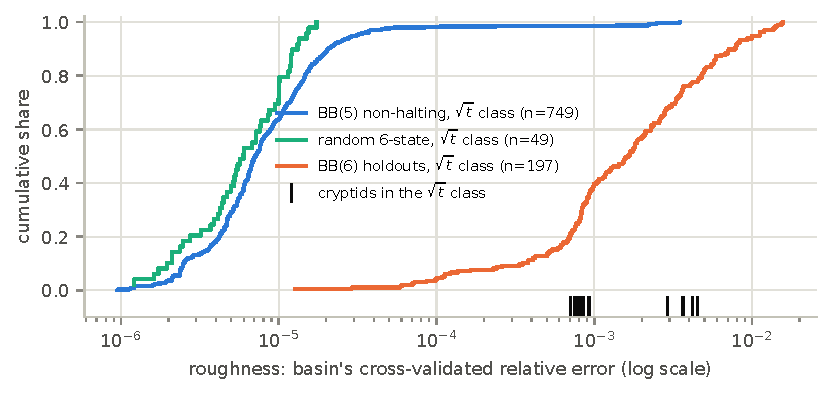
\includegraphics[width=\textwidth]{roughness}
\caption{Roughness within the $\sqrt t$ class: \BB{5} non-halting machines, random 6-state
machines and \BB{6} holdouts (cumulative distributions), with the cryptids as ticks. The holdouts
are separated from ordinary machines; the cryptids are not separated from other holdouts.}
\label{fig:roughness}
\end{figure}

Roughness therefore says that a machine is unusual, not in what way. The rest of the report asks
what makes a machine rough, starting with the one machine whose rule is fully known, the \BB{5}
champion.

%=================================================================================================
\section{The BB(5) champion: its constant from its rule}
\label{sec:champion}

The champion \tm{1RB1LC_1RC1RB_1RD0LE_1LA1LD_1RZ0LA} follows a Collatz-like rule (bbchallenge
wiki; Pascal Michel). With $C(n) = 0^\infty\,{<}A\,1^n\,0^\infty$ and the blank tape $C(0)$:
\[
C(3k) \to C(5k+6) \text{ in } 5k^2+19k+15 \text{ steps},\qquad
C(3k+1) \to C(5k+9) \text{ in } 5k^2+25k+27 \text{ steps},\qquad
C(3k+2) \to \text{halt}.
\]
The trajectory is $0, 6, 16, 34, \dots, 7366, 12284$, then halt. A tracer confirmed that at
every predicted time the tape has exactly the form $C(n)$, the span is $n+1$, and the machine
halts at 47,176,870.

\paragraph{Derivation.} Each macro step multiplies $n$ by about $5/3$ and costs about
$\tfrac59 n^2$ steps. Summing the geometric series gives $t \approx \tfrac5{16} n^2$ at each
configuration, so there
\[ \mathrm{span}/\sqrt t \to 4/\sqrt5 = 1.7889 \qquad(\text{measured } 1.7891). \]
Within a macro step the sub-rule $C(m, n) \to C(m+5, n-1)$ in $2m+8$ steps gives
$m\approx\sqrt{5\tau}$ and $\mathrm{span} \approx N + \tfrac25 m$ a time $\tau$ into a step that
starts at $C(N)$, so with $s = \sqrt\tau/N$
\[ \frac{\mathrm{span}}{\sqrt t} = \frac{1 + (2/\sqrt5)\,s}{\sqrt{5/16 + s^2}} . \]
Its maximum is exactly 2, at $s = \sqrt5/8$, which is 22\% of the way through each step in
$\log t$ (measured peaks $2.0003$--$2.003$ at 21--25\%). One cycle is a factor $25/9 = 2.78$ in
time (measured $2.78$--$2.80$). The average over $\log t$ is $1.9236$, against \texttt{basin}'s
$1.920$ (Figure~\ref{fig:champion}).

This wobble is all of the champion's roughness (cross-validated error $1.5\times10^{-3}$, rougher
than 99\% of non-halting $\sqrt t$ machines). Macro steps that multiply the size by a fixed factor
make the growth repeat on a log scale; bouncers add a fixed amount per sweep and grow smoothly.
A residual that is periodic in $\log t$ is therefore a candidate signature of macro steps that
multiply the size, as in Collatz-like rules, and its period gives the multiplier.

\begin{figure}[t]
\centering
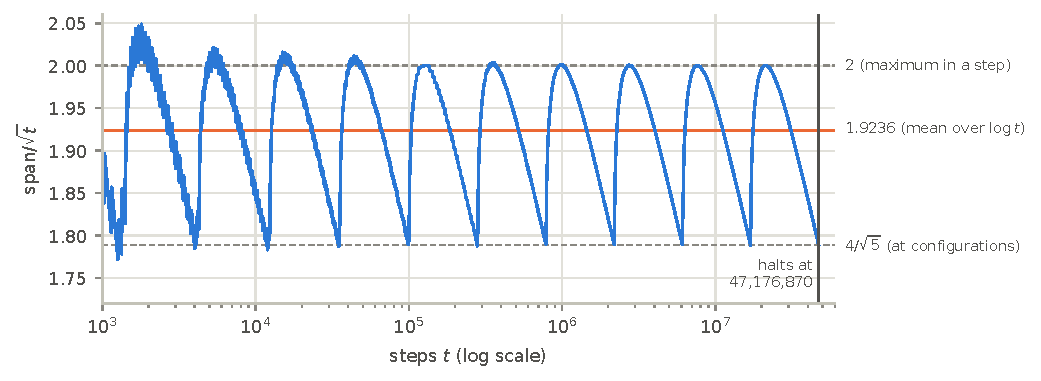
\includegraphics[width=\textwidth]{champion}
\caption{$\mathrm{span}/\sqrt t$ for the \BB{5} champion. It swings between $4/\sqrt5$ at
configurations and 2 within each macro step, once per factor $25/9$ in time; the mean over
$\log t$ is $1.9236$ and \texttt{basin}'s fitted constant is $1.920$.}
\label{fig:champion}
\end{figure}

%=================================================================================================
\section{A log-periodic wobble marks multiplicative rules}
\label{sec:wobble}

\subsection{Idea and prediction}
Section~\ref{sec:champion} showed that the champion's span wobbles around $c\sqrt t$ with a
period that is a fixed \emph{factor} of time, because each macro step multiplies the size by
$5/3$. In general, if a machine follows a rule $n \to \lambda n$ with span $\propto n$ and span
$\propto t^p$, the wobble repeats every factor $\lambda^{1/p}$ in time. A bouncer adds a fixed
amount per sweep, so its sweeps get closer together on a log scale and it has no such period.
Before looking at its data we predicted from Antihydra's published rule ($b \to \lfloor 3b/2\rfloor + 2$
or similar, depending on parity, at a cost of about $\tfrac34 b^2$ steps) a period of
$(3/2)^2 = 2.25$ in time, i.e.\ $\lambda = 3/2$.

\subsection{Method}
\begin{enumerate}
\item Simulate each machine to $2^{32}$ steps and record the span at 64 points per doubling of
$t$ (\texttt{wobble/spandense.c}).
\item On $t \ge 2^{12}$, fit $\ln \mathrm{span} = p\ln t + q$; the residual is the wobble.
\item For 600 trial periods $P$ (in $\ln t$) fit three harmonics to the residual and keep the
period with the largest share $R^2$ of residual variance explained.
\item A \emph{detection} is $R^2 > 0.5$ with at least four full cycles in the window (time factor
$e^P < 32$).
\item Refine $P$ on a fine grid and measure $\lambda$ directly, as the median ratio of the span at
successive minima of the wobble (one minimum per cycle, first cycle dropped). This second
estimate does not depend on the fitted exponent.
\end{enumerate}
The machines were the 608 holdouts, the 20 cryptids and 6 potential cryptids, the \BB{6}
champion, the 20 \BB{5} top halters, and as controls 200 random $\sqrt t$ machines from the \BB{5}
census, the 4 \BB{5} $t^{1/3}$ machines and the 49 random 6-state $\sqrt t$ machines.

\subsection{Results}
\begin{figure}[t]
\centering
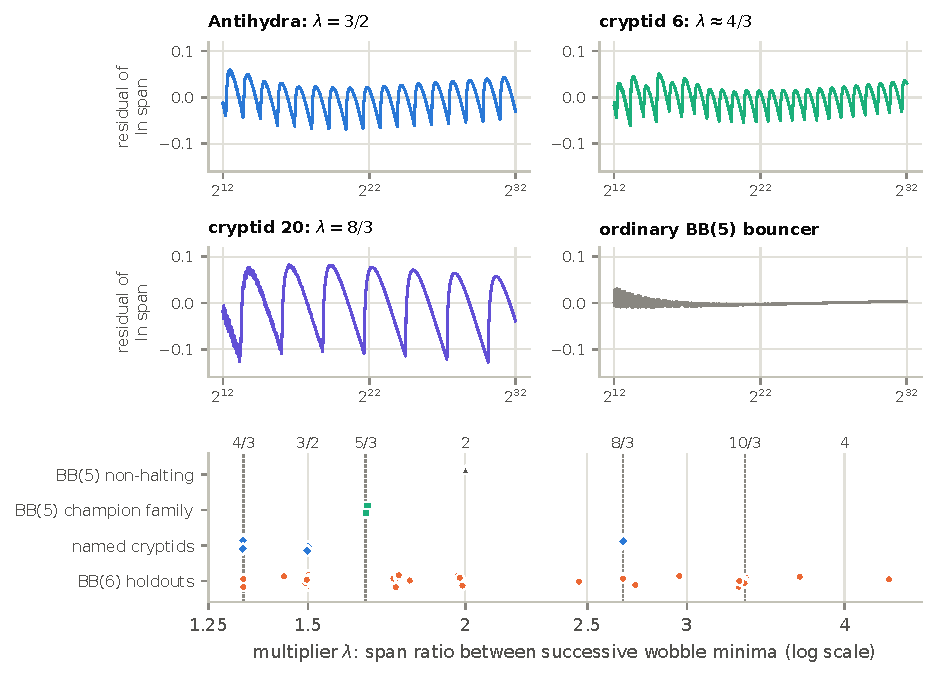
\includegraphics[width=\textwidth]{wobble}
\caption{Top: residual of $\ln\mathrm{span}$ after a straight-line fit in $\ln t$, for three
cryptids and an ordinary \BB{5} bouncer. Bottom: the multiplier $\lambda$ (span ratio between
successive wobble minima) for every detection; dashed lines mark simple fractions.}
\label{fig:wobble}
\end{figure}

Figure~\ref{fig:wobble} shows example residuals and every measured multiplier.
\begin{itemize}
\item \textbf{Controls are quiet.} The ordinary \BB{5} $\sqrt t$ machines have median
$R^2 = 0.10$ (90th percentile $0.18$) and the random 6-state $\sqrt t$ machines at most $0.18$.
One of the 200 \BB{5} machines, \tm{1RB0LC_1LC1LE_1RD0LB_0RA1RC_---0RA}, is detected
($R^2 = 0.91$); its span ratio between minima is $2.0000$, so a machine whose size doubles at
every macro step is hiding in the $\sqrt t$ class. Its rule, read from the tape in
Section~\ref{sec:rulecheck}, is $n \to 2n + 7$.
\item \textbf{The \BB{5} champion family} is detected in 19 of the 20 top halters ($R^2\approx0.93$),
with $\lambda = 1.672$ (champion) and $1.669$, against the known $5/3$.
\item \textbf{Antihydra confirms the prediction}: period factor $2.251$ (predicted $2.25$), and span
ratios between minima of $1.5000, 1.5001, 1.5000, 1.5001, 1.5005$ in its last cycles.
\item \textbf{Seven of the 20 cryptids are detected}, all with simple multipliers:
$3/2$ (Antihydra, cryptids 3 and 14; minima ratios $1.4983$--$1.5000$), $\approx4/3$ (cryptids 4 and 6;
$1.3316$--$1.3321$, $0.1\%$ below $4/3$) and $8/3$ (cryptids 13 and 20; $2.6657$, $2.6693$).
Cryptids 5 and 8 show the $4/3$ and $3/2$ periods but below the detection threshold.
\item \textbf{44 of the 608 holdouts are detected.} By nearest fraction (within 0.5\%):
$3/2$: 13, $10/3$: 4, $4/3$: 2, $8/3$: 2, $7/4$: 2, $9/5$: 2, $13/3$: 1, and 18 with no simple fraction
(several near $1.98$, possibly a slowly converging 2). Some of these may be equivalent forms of
named cryptids, since the holdout list uses its own normal form.
\item \textbf{The rest are not detected}, including Lucy's Moonlight, Space Needle, cryptids 9--12
and 15--19, all potential cryptids and the \BB{6} champion. The detector needs every branch of
the rule to multiply by the same factor; rules whose multiplier depends on parity (for example
$\times3/2$ in one branch and $\times1/2$ in another) give a wobble that is not periodic.
\end{itemize}

So a periodic wobble in $\log t$ is a specific signature of machines whose macro steps multiply
the size by a uniform factor, and its period measures the factor to about $0.1\%$ without knowing
the rule. It does not say whether the rule is Collatz-like, that is, whether it splits into cases
by residue; Section~\ref{sec:rulecheck} reads that off the tape.
Halting status is not visible in it: the $8/3$ cryptids are probviously halting and the $4/3$ ones
probviously non-halting, while $3/2$ occurs in both.

%=================================================================================================
\section{Cryptid rules from the tape, and a scale-invariance test}
\label{sec:cryptids}

The periodic-wobble detector of Section~\ref{sec:wobble} finds only rules that multiply by the same
factor on every branch. This section measures the multipliers of the other cryptids, checks them
against the machines' rules, and tests a more general signature.

\subsection{Teeth of the wobble}
Almost every cryptid's residual (Section~\ref{sec:wobble}) is a sawtooth: the span jumps at each
macro step and then relaxes. A \emph{tooth} is a sharp minimum of the residual (found with a
prominence of $0.25$ of the residual's 5--95\% range). For a rule $n \to \lambda n + O(1)$ the
span ratio between successive teeth converges to $\lambda$, whether or not the teeth are evenly
spaced in $\log t$. Measured ratios in the last cycles:
\begin{itemize}
\item $3/2$: Antihydra and cryptids 3, 8, 9, 10, 11, 12, 14, 15 (ratios settle at $1.499$--$1.500$;
cryptids 9 and 10 also show one large jump, $\times8.9$ and $\times12.8$);
\item $4/3$: cryptids 4, 5, 6 ($1.331$--$1.332$);
\item $8/3$: cryptids 13 and 20, and Lucy's Moonlight ($2.525, 2.621, 2.649, 2.662, 2.665$);
\item mixed ratios: cryptids 16, 17, 19 and Space Needle (values such as $1.25$, $1.5$, $1.9$,
$3.2$--$5.0$);
\item tiny ratios ($1.03$--$1.2$): potential cryptids 3--6, which grow like $t^{1/3}$.
\end{itemize}

\subsection{Rules read from macro configurations}
To check these numbers against the machines' actual rules, the tape is recorded at every visit of
the head to an edge of the visited region, with edge zeros trimmed, and compressed into
\emph{tokens}: a unit of 1 to 4 cells repeated three or more times becomes $(u)^k$
(\texttt{collatz/macro2.py}). The token list with exponents replaced by $n$ is the tape's
\emph{shape}. For the most visited (state, side), runs of identical shapes are the sub-steps of a
macro step, and shape changes mark the macro steps. Applied to Antihydra this recovers its
published configuration $1^a\,0\,1^b$ (state E at the right edge) and its rule; for example
$b = 131 \to (3\cdot131+3)/2 = 198$ with $a$ falling by 1, and $b = 198 \to 3\cdot198/2 + 2 = 299$.

\begin{table}[t]
\centering\small
\begin{tabular}{@{}p{2.6cm}p{2.2cm}p{9.4cm}@{}}
\toprule
cryptid & multiplier & evidence from macro configurations \\
\midrule
Antihydra & $3/2$ & published rule; $1^a\,0\,1^b$ with $b \to (3b+3)/2$ ($a-1$) or $3b/2+2$ ($a+2$)\\
Lucy's Moonlight & $8/3$ & published rule: $C(a{+}1, 3k) \to C(a, 8k{+}6)$ and similar; a reset branch sets $b = 8$\\
4 & $4/3$ & $(10)^x\,(110)^y\,11$ at boundaries, $x = 871 \to 1163 \to 1552 \to 2071 \to 2763$, i.e.\ $x \to (4x{+}5)/3$ or $(4x{+}4)/3$ by $x \bmod 3$; $y$ grows by 1 per step\\
5, 6 & $4/3$ & main block $2090 \to 2791 \to 3723 \to 4970$ and $2443 \to 3259 \to 4347 \to 5802$; a second variable changes by $+4$, $+6$ or $-1$, like Antihydra's $a$\\
8, 9, 10, 11, 12, 15 & $3/2$ & e.g.\ cryptid 11: $1300 \to 1954 \to 2935 \to 4408$ with a side counter $6 \to 5 \to 4 \to 3$, after which the shape changes (the large jump in its wobble near $2^{26.5}$); cryptid 12: $811 \to 1222 \to 1840 \to 2764$ with $41 \to 39 \to 37 \to 35 \to 33$\\
13, 20 & $8/3$ & within a step one unary block loses 3 cells per 4 units gained by a $(01)$ block; at 2 cells per unit this is $2 \times 4/3$\\
16 & $3/2$, $5/4$ & $1^n$: odd $n \to (3n+3)/2$ (e.g.\ $477 \to 717 \to 1077 \to 1617 \to 2427 \to 3642$); $n \equiv 0 \pmod 4 \to (5n+8)/4$ ($104 \to 132 \to 167$, $252 \to 317$)\\
17 & $3/2$, $9/8$ & boundaries $1367 \to 1540 \to 2312 \to 3470$; in the $9/8$ branch the block splits $3{:}1$ and only the quarter is multiplied by $3/2$\\
19 & $3/2$, $5/4$, ($9/8$) & $1^n$: even $n \to (3n+4)/2$; $n \equiv 1 \pmod 4 \to (5n+11)/4$ ($185 \to 234$, $353 \to 444$); one example $71 \to 80$\\
Space Needle & none & $1^a\,0\,1^b\,0\,1^c$: $a$ is moved into $b$ at two cells per cell while $c$ is unchanged, so the growth per step depends on $a{:}b$; $\mathrm{span}\propto t^{0.35}$\\
18 & -- & one macro step in the window\\
\bottomrule
\end{tabular}
\caption{Multipliers of the \BB{6} cryptids and the rule evidence for each
(\texttt{results/cryptid\_multipliers.csv}). The multipliers of Lucy's Moonlight and Antihydra are
from the bbchallenge wiki; the others were derived here.}
\label{tab:cryptidrules}
\end{table}

Every multiplier predicted from the wobble agrees with the rule (Table~\ref{tab:cryptidrules}).
The ``mixed'' teeth come from rules whose multiplier depends on a residue, for example $3/2$ for
odd $n$ and $5/4$ for $n \equiv 0 \pmod 4$.

\subsection{Scale invariance: the wobble does not decay}
If macro steps multiply the size, the configuration at each step is a scaled copy of the previous
one, so the relative wobble of the span about its power law keeps the same size at every scale.
If growth is additive (a bouncer gains a fixed number of cells per sweep), the wobble is about one
cell and its relative size falls like $1/\mathrm{span} \propto t^{-p}$.

\paragraph{Statistic.} Take the residual of $\ln\mathrm{span}$ after a straight-line fit in
$\ln t$, remove slow trends by subtracting a running mean over two octaves, and compare its
standard deviation in an early and a late window: $D = \log_2(\sigma_\text{late}/\sigma_\text{early})$.
For a wobble of one cell, $D = -p\,g$ where $g$ is the distance in octaves between the window
centres. The index $S = D/(-p\,g)$ is about 1 for additive growth and about 0 for scale-invariant
growth (\texttt{collatz/decay.py}, \texttt{screen/scalestat.py}).

\paragraph{Results.} With the $2^{32}$ runs (windows $2^{13}$--$2^{18}$ and $2^{26}$--$2^{31}$,
$g = 13$) the predicted decay was confirmed before any Collatz-like machine was examined: BB(5)
$\sqrt t$ machines $D = -6.50$ (predicted $-6.5$), random 6-state $\sqrt t$ machines $-6.52$,
BB(5) $t^{1/3}$ machines $-4.33$ (predicted $-4.33$).

\begin{table}[h]
\centering\small
\begin{tabular}{@{}lrrrr@{}}
\toprule
set & $n$ & $S > 0.75$ (fades as $1/\mathrm{span}$) & $0.25$--$0.75$ & $S < 0.25$ (scale-invariant)\\
\midrule
BB(5) $\sqrt t$ (random) & 200 & 199 & 0 & 1\\
random 6-state $\sqrt t$ & 49 & 49 & 0 & 0\\
BB(5) $t^{1/3}$ & 4 & 4 & 0 & 0\\
\BB{6} cryptids & 20 & 0 & 1 & 19\\
potential cryptids & 6 & 0 & 4 & 2\\
\BB{6} holdouts, $p \in (0.4, 0.6]$ & 449 & 32 & 59 & 358\\
\BB{6} holdouts, $p \in (0.2, 0.4]$ & 53 & 5 & 45 & 3\\
\bottomrule
\end{tabular}
\caption{Scale-invariance index on the $2^{32}$ runs. The one scale-invariant BB(5) machine is the
$\lambda = 2$ machine of Section~\ref{sec:wobble}. The cryptid in the middle band is cryptid 18,
which has a single macro step in the window. Holdouts with $p \le 0.2$ (mostly $\log t$) are left
out, because $S$ divides by $p$.}
\label{tab:decay}
\end{table}

Table~\ref{tab:decay} gives the results. Two points stand out. Cryptids and 80\% of the $\sqrt t$-like holdouts are scale-invariant, while
ordinary bouncers are not. And a third group, the $t^{1/3}$-like holdouts and potential cryptids
3--6, decays about halfway ($S \approx 0.5$) and has many small teeth; its mechanism is not
known. Scale invariance describes how a machine grows, not whether it halts: the $\lambda = 2$
\BB{5} machine is scale-invariant and proven non-halting.

With the shorter $2^{26}$ window used for the \BB{5} screen (Section~\ref{sec:screen}) (windows $2^{13}$--$2^{18}$ and
$2^{20.5}$--$2^{25}$, $g = 7.25$), the same machines give the same separation: all 20 cryptids
(including cryptid 18) have $S < 0.25$, 199 of the 200 BB(5) bouncers and all 49 random 6-state
bouncers have $S > 0.75$.

%=================================================================================================
\section{Screening BB(5) for scale-invariant machines}
\label{sec:screen}

How common is scale invariance among ordinary machines? The statistic of Section~\ref{sec:cryptids}
was applied to the $\sqrt t$-like part of the \BB{5} database.

\paragraph{Data and method.} All 14,322,029 time-limit records of the \BB{5} database were run for
$2^{16}$ steps; the 2,767,634 records whose span slope between $2^{14}$ and $2^{16}$ lies in
$[0.4, 0.6]$ are the $\sqrt t$-like population. Every one of them was run to $2^{26}$ steps,
recording the span at 16 points per octave (\texttt{screen/screen.c}), and scored with the $2^{26}$
statistic; the $2^{24}$ statistic was computed from the first 225 points of the same rows. A
uniform sample of 300,000 records (seed 0) was run and analysed first, and its estimate recorded
before the other 2,467,634 were run. The same run included 71 controls: the 20 cryptids, 6
potential cryptids, the \BB{6} champion, the $\lambda = 2$ machine and Skelet's 43 machines
(\texttt{results/screen\_controls\_2e26.csv}).

\paragraph{Result.} The index is sharply bimodal: 2,732,054 records (98.71\%) fade like
$1/\mathrm{span}$, \textbf{34,956 (1.263\%) are scale-invariant}, and only 624 fall in between
(\texttt{results/bb5\_screen\_full\_scores.csv.gz}). The 300,000-record sample had predicted
$1.27\% \pm 0.04\%$, or $35{,}250 \pm 1{,}100$ records; the other 2,467,634 records give $1.262\%$.
The share varies along the database, from $0.87\%$ to $1.74\%$ across tenths of the index range,
so a run stopped part way through in index order would have been biased; the uniform sample was
not.

\paragraph{The label does not depend on the window.} Scored on $2^{24}$ steps instead of $2^{26}$,
the same rows give the same class for 99.992\% of records. Of the 34,956 scale-invariant records,
34,926 are scale-invariant on both windows; in all, 213 records change class, almost all between
the intermediate band and one of the other two.

\paragraph{Multipliers.} The 34,956 records have 16,347 distinct span sequences (11,118 of them
occur as a single record, and 13,326 were not in the sample). Their multipliers, from the span
ratio between successive teeth (\texttt{results/bb5\_screen\_full\_scaleinv.csv}):

\begin{center}\small
\begin{tabular}{@{}lrr@{}}
\toprule
multiplier from the teeth & distinct behaviours & records\\
\midrule
2 & 11,489 & 27,540\\
3/2 & 2,172 & 3,221\\
4/3 & 203 & 254\\
3 & 180 & 351\\
4 & 140 & 233\\
5/2 & 36 & 40\\
5/3 & 16 & 18\\
5/4 & 16 & 17\\
8/3 & 3 & 3\\
other fractions (8/7, 7/4, 10/7, 6/5, 12/7, \dots) & 95 & 124\\
no simple fraction & 1,997 & 3,155\\
\midrule
total & 16,347 & 34,956\\
\bottomrule
\end{tabular}
\end{center}

The multipliers $5/3$ and $8/3$, those of the champion and of cryptids 13 and 20, do not occur in the
300,000-record sample at all. A teeth ratio is a measurement, not a rule; Section~\ref{sec:fullrules}
reads the rules of these behaviours from their tapes.

Reading the tapes of examples (with the method of Section~\ref{sec:rulecheck}) shows two kinds:
\begin{itemize}
\item \textbf{Doubling bouncers} ($\lambda = 2$). For example record 6,503,294
(\tm{1RB0LC_0LC1LB_1RD1LA_1RE---_1RB0RA}) goes $1^{2042} \to 1\,(10)^{1022}\,1 \to \dots \to 1^{4090}$,
that is $n \to 2n + 6$ every time. There is no case split, so the scale invariance is real but the
dynamics are simple.
\item \textbf{Collatz-like machines} ($\lambda = 3/2$). For example record 4,823,469
(\tm{1RB0RC_1LC1RB_---1LD_1LE1RE_1LA0RD}) starts each counting phase with the tape
$1^n\,(01)^4$, and over 13 macro steps ($395 \to 598 \to 902 \to \dots \to 4607 \to 6916$)
\[ n \to \tfrac32 n + 5 \ \ (n \text{ even}), \qquad n \to \tfrac{3n + 11}{2} \ \ (n \text{ odd}) \]
exactly. Records 5,644,960 and 3,270,527 follow rules of the same form.
\end{itemize}
Two examples whose teeth gave no simple fraction are exact $\times4$ and $\times3$ rules
($n \to 4n + 22$ and $n \to 3n + 16$) that the teeth had not resolved.

\paragraph{Skelet's machines.} Seven of the 43 are scale-invariant: Skelets 1, 16, 19, 24, 38, 40
and 42. Six of these (16, 19, 24, 38, 40, 42) are exactly the power-law machines among the seven
Skelets that the Coq-BB5 proof decided with its \texttt{TABLE\_BASED\_DNV} certificates; the
seventh, Skelet 9, grows logarithmically and cannot be scored. Skelet 1, a translated cycler whose
cycle starts only after about $5.4\times10^{51}$ steps, is scale-invariant during its long
pre-period. The bouncers (Skelets 20, 21, 28, 39) and Skelet 17 fade like $1/\mathrm{span}$.
Skelets 3, 7, 23 and 29 fall in the intermediate band, with the $t^{1/3}$-like holdouts.
Section~\ref{sec:rulecheck} reads the Skelets' rules from their tapes.


%=================================================================================================
\section{Counters or Collatz maps? Rules read from the tape}
\label{sec:rulecheck}

A wobble that keeps its size says that a machine's macro steps multiply its size. It does not say
what kind of rule does the multiplying. A rule $n \to 2n + 6$ is scale-invariant but is an
exponential counter: one formula, applied forever. A Collatz-like rule needs a different formula
for each residue of $n$, as in the champion's $C(3k) \to C(5k+6)$, $C(3k+1) \to C(5k+9)$,
$C(3k+2) \to$ halt. This section reads which kind a machine follows from its tape, for the control
machines and for the \BB{5} census machines that \texttt{basin} fitted.

\subsection{Method}
\begin{enumerate}
\item Run the machine for $2^{26}$ steps (\texttt{collatz/macroc.c}). At each visit of the head to
an edge, in the (state, side) visited most often in the second half of the run, compress the tape
into a shape as in Section~\ref{sec:cryptids} and keep one record per run of identical shapes.
\item For every shape with one to three repeated blocks, take the block lengths at each new
occurrence of the shape. Successive occurrences give transitions $n_k \to n_{k+1}$ for each block.
Keep blocks that grow in at least 75\% of the transitions, with at least three transitions from
$n_k \ge 20$.
\item Fit the slope by least squares and snap it to the nearest fraction $p/q$ with $q \le 8$
(within 2\%). Then, using exact integer arithmetic with no tolerance, call the rule
\begin{itemize}
\item \emph{additive} if $p/q = 1$ and $n_{k+1} - n_k$ is constant;
\item \emph{one formula} if $p/q \ne 1$ and $q\,n_{k+1} - p\,n_k$ is the same for every transition;
\item \emph{by residue} (Collatz-like) if it is not, but for some $d \le 6$ it is constant within
each class of $n_k \bmod d$ (at least two classes with two transitions each);
\item \emph{irregular} otherwise.
\end{itemize}
\item Report the block with an exact rule, preferring multiplicative rules to additive ones and then
the widest range of $n$ (\texttt{collatz/macrorule.py}; results in \texttt{results/macro\_rules.csv}).
\end{enumerate}
\paragraph{Which rules are Collatz-like.} A fractional multiplier $p/q$ forces a case split, because
$\tfrac pq n$ is a whole number only when $q$ divides $n$. A growing orbit also cannot follow a
fixed repeating pattern of cases forever. A pattern of length $P$ composes to a single map
$n \to (p/q)^P n + c$, and the only number that follows the pattern for ever is that map's fixed
point (the same argument limits cycles in the Collatz problem), so a growing orbit must break the
pattern. An integer multiplier allows one formula, or a fixed repeating pattern of formulas, which
over one period is again one formula. So a rule is called \emph{Collatz-like} when its multiplier
is fractional, and an \emph{exponential counter} when the multiplier is an integer and the rule
is one formula or a repeating pattern of them. Both halves of the argument hold in the data
(Section~\ref{sec:fullrules}).

A short run can see a fractional rule on only one residue class. For example
\tm{1RB---_1RC0RA_1LD0RB_0LE0LC_1RA0LE} goes $52 \to 152 \to 402 \to 1027$ by
$n \to \tfrac52 n + 22$, all from even $n$, and the window ends at the odd value 1027. Such rules
count as Collatz-like by their multiplier.

\subsection{Validation on machines with known rules}
\begin{table}[h]
\centering\small
\begin{tabular}{@{}p{4.3cm}p{4.4cm}p{5.4cm}@{}}
\toprule
machine & rule read from the tape & check \\
\midrule
\BB{5} champion & $\times5/3$, by $n \bmod 3$ & published rule (Section~\ref{sec:champion})\\
Antihydra & $\times3/2$, by parity & published rule\\
cryptids 3, 8, 11, 14 & $\times3/2$, by $n \bmod 2$ or $4$ & Table~\ref{tab:cryptidrules}\\
cryptids 4, 5, 6 & $\times4/3$, by $n \bmod 3$ & Table~\ref{tab:cryptidrules}\\
cryptid 20 & $\times8/3$, by $n \bmod 3$ & Table~\ref{tab:cryptidrules}\\
cryptids 9, 10, 15; 16, 17, 19; Lucy's Moonlight & $\times3/2$; $\times5/4$; $\times8/3$, no
exact formula & multipliers agree; these rules switch branches or carry a second counter, so
successive occurrences of one shape are not one macro step apart\\
cryptids 12, 13, 18, Space Needle, potential cryptids, \BB{6} champion & unresolved & too few
transitions, or no recurring shape with at most three blocks\\
$\lambda = 2$ machine (Section~\ref{sec:wobble}) & $n \to 2n + 7$ & wobble $\lambda = 2.0000$\\
screen examples, $\lambda = 2$ (2) & $n \to 2n + c$, one formula each & teeth $\lambda = 2$\\
screen examples, $\lambda = 3/2$ (3) & $\times3/2$, by parity & teeth $\lambda = 3/2$\\
screen examples, no fraction (2) & $n \to 3n+16$, $n \to 4n + 22$ & teeth near 3 and 4\\
\bottomrule
\end{tabular}
\caption{The rule test on machines whose rules or multipliers are known. Every exact rule found
agrees with the published rule or the measured multiplier.}
\label{tab:rulecheck}
\end{table}

The test recovers the champion's and Antihydra's published rules, and confirms the cryptid
multipliers of Table~\ref{tab:cryptidrules} as exact residue rules for nine cryptids
(Table~\ref{tab:rulecheck}). It fails safe: where it cannot find an exact rule it says so, and
none of its exact rules contradicts a known one.

\subsection{Skelet's machines}
\begin{itemize}
\item \textbf{The six scale-invariant power-law Skelets are doublers.} Skelets 16, 19, 24, 38, 40
and 42 each follow one exact formula; Skelets 19 and 42 run through $15, 31, 63, \dots, 2047$
($n \to 2n + 1$). They are exponential counters, not Collatz-like machines.
\item \textbf{Skelets 9, 23 and 29 are additive} ($n \to n + 4$, $n + 2$, $n + 2$).
\item \textbf{Skelet 17 has no multiplicative rule.} It was one of the last \BB{5} holdouts and needed
an individual proof in Coq-BB5. Its tape holds a growing list of numbers that it updates like a
Gray-code counter (bbchallenge wiki), so no shape with three or fewer blocks recurs, and its
wobble fades like a bouncer's ($S = 1.10$). The hardest machine in \BB{5} is hard for a reason
that has nothing to do with Collatz-like rules.
\item Of the rest, 31 have no recurring shape with at most three blocks (seven of them because
their tapes grow past $10^5$ cells, which the test skips), Skelets 4 and 37 are irregular, and
Skelet 36 settles to a fixed size.
\end{itemize}

\subsection{The whole \BB{5} screen}
\label{sec:fullrules}
The test was run on one representative of every distinct scale-invariant behaviour of the full
screen whose teeth gave a multiplier other than 2: 2,861 behaviours, all of the $3/2$ group and
everything rarer (\texttt{results/bb5\_screen\_tape\_rules.csv}). Table~\ref{tab:fullrules} and
Figure~\ref{fig:screenrules} give the result.

\begin{table}[h]
\centering\small
\begin{tabular}{@{}llrr@{}}
\toprule
rule read from the tape & multiplier & distinct behaviours & records\\
\midrule
Collatz-like (fractional, by residue) & $3/2$ & 2,026 & 3,002\\
 & $4/3$ & 117 & 150\\
 & $5/2$ & 29 & 33\\
 & $5/4$ & 12 & 13\\
 & $5/3$ & 5 & 5\\
 & $7/4$ & 5 & 5\\
 & $8/3$ & 2 & 2\\
exponential counter (integer, one formula) & $3$ & 190 & 367\\
 & $4$ & 148 & 241\\
 & $2$ & 32 & 45\\
 & $5$, $6$ & 3 & 6\\
additive & 1 & 8 & 8\\
unresolved & & 284 & 384\\
\midrule
total read & & 2,861 & 4,261\\
not read: teeth $\lambda = 2$ & & 11,489 & 27,540\\
not read: no simple fraction from the teeth & & 1,997 & 3,155\\
\bottomrule
\end{tabular}
\caption{Rules of the scale-invariant \BB{5} behaviours, read from the tape. The $3/2$ row includes
22 behaviours whose followed shape recurs only every second macro step, so the test read
$(3/2)^2 = 9/4$.}
\label{tab:fullrules}
\end{table}

\begin{figure}[t]
\centering
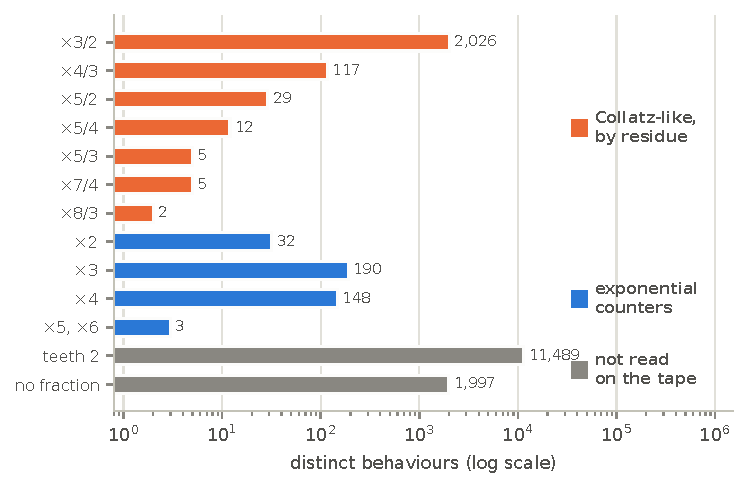
\includegraphics[width=0.8\textwidth]{screenrules}
\caption{Distinct scale-invariant \BB{5} behaviours by the rule read from the tape (log scale).
Collatz-like rules occur with every multiplier found in the cryptids and the champion except
$9/8$; exponential counters have integer multipliers. The largest group, teeth ratio 2, was not
read on the tape.}
\label{fig:screenrules}
\end{figure}

\begin{itemize}
\item \textbf{2,196 distinct behaviours (3,210 records) are Collatz-like}, with multipliers $3/2$,
$4/3$, $5/2$, $5/4$, $5/3$, $7/4$ and $8/3$. Every multiplier of the cryptids and the champion
except cryptid 17's $9/8$ occurs among these proven non-halting \BB{5} machines. Of the 2,172
behaviours with teeth near $3/2$, 2,026 are confirmed Collatz-like.
\item \textbf{373 behaviours (659 records) are exponential counters} with multiplier 2, 3, 4, 5 or
6. Teeth near 3 or 4 are almost always counters ($177$ of $180$ and $138$ of $140$; the rest are
unresolved), and so are most
odd teeth ratios such as $23/8$ or $25/6$, which turn out to be $\times3$ and $\times4$ rules the
teeth had misread.
\item \textbf{The case-pattern argument holds.} The three integer-multiplier rules that do split
into cases repeat their cases with period 2: for example $11 \to 44 \to 137 \to 422 \to 1271$
alternates $n \to 3n + 11$ (odd $n$) and $n \to 3n + 5$ (even $n$), which is $n \to 9n + 38$ over
two steps. Of the 2,196 fractional rules, 2,158 visit more than one residue class, and none of these repeats
its cases within the window (the other 38 were seen on one class only, as in the example above); the residues
of the $\times8/3$ machine \tm{1RB0LE_1RC0LA_1LD0RA_---1LE_1LB0LB}, for example, run
$0, 2, 1, 1, 0, 2$ (mod 3) as $n$ goes $12, 44, 130, 358, 966, 2588$.
\item \textbf{Not read:} the 11,489 behaviours with teeth ratio 2 and the 1,997 with no simple
fraction. Every $\times2$ example read so far (in the sample, the census and among the Skelets) is a
doubler, and the unmatched examples were $\times3$ and $\times4$ counters, so these are probably
mostly counters, but this has not been checked machine by machine.
\end{itemize}

So among the 34,956 scale-invariant \BB{5} records, at least 3,210 (9\%) follow Collatz-like rules
and at least 659 are exponential counters; the unread $\times2$ group makes up most of the rest.

\subsection{\texttt{basin}'s roughness sees the same machines}
The 638 time-limit $\sqrt t$ machines in the \BB{5} census sample of Section~\ref{sec:classes} were
run to $2^{26}$ steps and scored for scale invariance, and the scale-invariant and roughest ones
were read on the tape (Figure~\ref{fig:rulecheck}; \texttt{results/bb5\_census\_sqrt\_scaleinv.csv},
\texttt{screen/census\_compare.py}).

\begin{figure}[t]
\centering
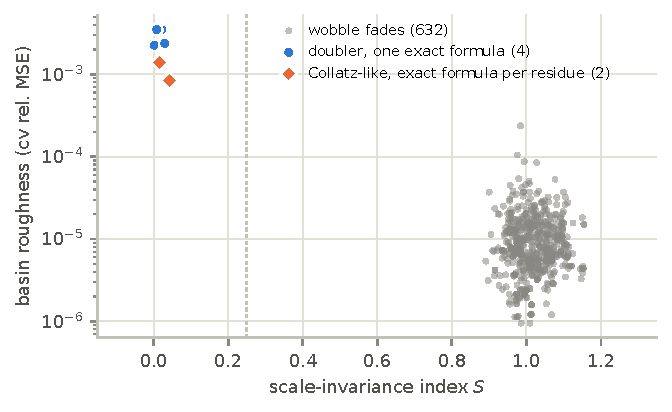
\includegraphics[width=0.72\textwidth]{rulecheck}
\caption{\texttt{basin}'s roughness against the scale-invariance index for the 638 time-limit
$\sqrt t$ machines of the \BB{5} census sample, coloured by the rule read from the tape. The six
scale-invariant machines are the six roughest fits.}
\label{fig:rulecheck}
\end{figure}

\begin{itemize}
\item 632 fade like $1/\mathrm{span}$, 6 are scale-invariant, none lie between.
\item \textbf{The six roughest fits are exactly the six scale-invariant machines} (AUC $1.000$,
Mann--Whitney $p = 2\times10^{-5}$). The least rough of them ($8.4\times10^{-4}$) is $3.5\times$
rougher than the roughest machine that fades ($2.4\times10^{-4}$); the median machine that fades
is at $7\times10^{-6}$.
\item On the tape, four are doublers (for example $94 \to 190 \to 382 \to \dots \to 12286$, that
is $n \to 2n + 2$; one of the four is the $\lambda=2$ machine of Section~\ref{sec:wobble}). One,
\tm{1RB1RE_1LC1LE_1RD1LC_---0RA_1RA0LB}, is $\times5/3$ by $n \bmod 3$, the same kind of rule as the
champion. One, \tm{1RB1LC_1RC---_0RD0LA_0RE1RC_1LE0LC}, is $\times3/2$ by parity.
\item Of the next nine roughest machines, seven grow additively on the tape ($n \to n + c$ with
$c = 2$ to $10$) and two have no recurring shape.
\end{itemize}

So on ordinary \BB{5} machines three different measurements pick out the same machines: a rough
\texttt{basin} fit, a wobble that keeps its size, and a macro rule that multiplies. This is the
mechanism behind the champion's roughness in Section~\ref{sec:champion}, now seen across a
uniform sample. Roughness does not, in principle, tell the two kinds apart, since both keep a
wobble of constant relative size; here the two Collatz-like machines happen to be the least
rough of the six, but six machines are too few to say whether that holds generally.

Among the \BB{6} holdouts the link is looser. Almost every holdout is rough
(Section~\ref{sec:bb6}), including those whose wobble fades: the median roughness of the
scale-invariant $\sqrt t$ holdouts is $2.0\times10^{-3}$, against $1.4\times10^{-3}$ for those
that fade, and the rank correlation between $S$ and roughness is only $-0.38$ ($\sqrt t$),
$-0.33$ ($\log t$) and $-0.31$ (\emph{other}). Among hard machines, roughness has other sources,
such as having no clean law at all.

\subsection{Proof difficulty is a different question}
Every \BB{5} machine has been proven non-halting, and bbchallenge publishes which stage of its
pipeline decided each record. Of the 345 $\times3/2$ records in the screen sample, 341 were decided
by generic deciders (243 by backward reasoning, 74 by halting segment, 24 by finite automata
reduction). These prove that the halting transition can never be reached from local or
automaton-based arguments, without using the machine's macro rule; only 4 reached the final
Coq-BB5 stage. Conversely, Skelet 17 is among the hardest
machines and is not multiplicative. Whether a machine is Collatz-like and whether its halting is
hard to decide are separate questions: a cryptid is the rare case of a Collatz-like rule in which
one branch leads to the halting transition, so that halting depends on the rule's long-run
behaviour.


%=================================================================================================
\section{Limits and open questions}
\begin{itemize}
\item \textbf{Window.} Every class and constant describes $2^{12}$--$2^{22}$ steps. Rerunning to
longer windows matters most for the holdouts' $t^{1/3}$, $t^{2/3}$ and \emph{other} labels.
\item \textbf{Gaps between classes.} Raw slopes (no \texttt{basin}) for all 436,278 \BB{4}
machines and a million \BB{5} machines would bound the empty slope ranges far better than the
20,000 samples.
\item \textbf{Counting bases.} Apply the weight regression to every counter, including the
unidentified ones and the $2^{4/9}$ cluster; resolve the restarting $3/2$ machines; look for a
counter in an irrational non-Pisot base (a Salem number, say), which would refute the refined
hypothesis.
\item \textbf{Bouncers.} Derive $c^2 = ah$ from the transition table for a few machines and check
it against the fitted $c$.
\item \textbf{Collatz-like machines.} Read the tapes of the two unread groups of the \BB{5} screen
(11,489 behaviours with teeth ratio 2 and 1,997 with no simple fraction), to count counters and
Collatz-like machines exactly; screen the space-limit records and the other growth classes, which
the screen left out; run the test on the \BB{6} holdouts. Extend it to
rules that switch branches or carry a second counter (cryptids 9, 10, 15--17, 19, Lucy's
Moonlight) by following the macro step itself instead of one shape. Derive Antihydra's constant
$1.377$ from its rule as was done for the champion. Find the mechanism of the group with
$S \approx 0.5$ (the $t^{1/3}$-like holdouts and potential cryptids 3--6).
\item \textbf{Share stability} across 3--5 states may partly reflect that larger trees contain
smaller machines with unused states; restricting to machines that visit every state would test
this.
\item \textbf{Baseline.} The random 6-state machines are uniform over transition tables, not over
the normal-form tree, so their class mix is not directly comparable to the \BB{3}--\BB{5} shares.
\end{itemize}

%=================================================================================================
\section{Reproducing}
\label{sec:repro}
Scripts live in \texttt{busy\_beaver/}; compile each \texttt{.c} file with
\texttt{gcc -O2 -o name name.c -lm}. Large intermediates are not committed and are regenerated by
the commands in \texttt{busy\_beaver/README.md}. \texttt{analyze.py} recomputes every census
number from \texttt{results/}. The base-$3/2$ analysis uses \texttt{pisot/weights.py},
\texttt{pisot/weights2.py} and \texttt{pisot/phasefit.py} (tape regression),
\texttt{pisot/incrlong.c} (long runs) and \texttt{pisot/converge.py}. The wobble analysis uses
\texttt{wobble/spandense.c}, \texttt{wobble/wobble.py}, \texttt{wobble/run\_wobble.py} and
\texttt{wobble/refine.py}. The cryptid rules and scale invariance use \texttt{collatz/teeth.py},
\texttt{collatz/macro2.py} and \texttt{collatz/decay.py}. The \BB{5} screen uses
\texttt{screen/screen.c}, \texttt{screen/score.py}, \texttt{screen/scalestat.py} and
\texttt{screen/multipliers.py} (the 300,000-record sample), \texttt{screen/run\_full.sh} and
\texttt{screen/finish\_tail.sh} (the full run), \texttt{screen/score\_all.py} and
\texttt{screen/multipliers\_all.py} (scoring all records); \texttt{screen/labels.py} attaches
bbchallenge's decider labels. The rule test uses \texttt{collatz/macroc.c} and \texttt{collatz/macrorule.py}, and the
comparison with \texttt{basin}'s census \texttt{screen/census\_compare.py}. The figures are made by
\texttt{report/figures.py}.

\section*{Sources}
\begin{itemize}\small
\item bbchallenge seed database: \url{https://docs.bbchallenge.org/}
\item Cryptids, BB(6), holdouts, BB(5), counters and the 5-state winner: \url{https://wiki.bbchallenge.org/}
\item Pascal Michel, the champion's behaviour: \url{https://bbchallenge.org/~pascal.michel/beh}
\item Skelet 17: \url{https://wiki.bbchallenge.org/wiki/Skelet_17}
\item Decider labels for the \BB{5} database: \url{https://docs.bbchallenge.org/bb5_decided_indexes/}
\item bbchallenge Collaboration, ``Determination of the fifth Busy Beaver value'', arXiv:2509.12337 (2025).
\item C.~Frougny, ``Representations of numbers and finite automata'', \emph{Mathematical Systems
Theory} 25 (1992) 37--60.
\item S.~Akiyama, C.~Frougny, J.~Sakarovitch, ``Powers of rationals modulo 1 and rational base
number systems'', \emph{Israel Journal of Mathematics} 168 (2008) 53--91.
\end{itemize}

\end{document}
